\documentclass[conference]{IEEEtran}

% --- Packages you might need ---
\usepackage[utf8]{inputenc}   % Encoding
\usepackage{amsmath,amssymb}  % Math symbols
\usepackage{graphicx}         % Figures
\usepackage{cite}             % Better citations
\usepackage{hyperref}         % Clickable links
\usepackage{algorithm}
\usepackage{algorithmic}
\usepackage{booktabs}
\usepackage{subcaption}
\usepackage{tabularx}   % For tables of a fixed width
\usepackage{ragged2e}   % For better text alignment (\RaggedRight)
\usepackage{comment}
\usepackage{float}

% --- Title and author ---
\title{Exploration of DyNA PPO with Dynamic Ensemble}

\author{
    \IEEEauthorblockN{Leihao (Eric) Lin\IEEEauthorrefmark{1}}
    \IEEEauthorblockA{\IEEEauthorrefmark{1}Department of Computer Science, Western University \\
    Email: llin286@uwo.ca}
}

\begin{document}

\maketitle

% Abstract
\begin{abstract}
This is the abstract of the paper. 
\end{abstract}


% introduction
\section{Introduction}
Introduction of the project
...



%Background and Related Works
\section{Backgrounds and Related Works}
Using PPO, a stable policy-gradient RL method to solve the black box optimization of biological sequence design. 
It proposes DyNA PPO, a variant of Proximal Policy Optimization:
\begin{itemize}
	\item Learns a surrogate reward model through supervised regression on data collected.
	\item Using cross validated R2, selects from a pool of candidate regressors whose predictions are above a threshold, and uses their ensemble average as a simulator for policy updates.
	\item Falls back to model-free PPO when no accurate surrogate is available, avoiding model bias.
	\item Adds exploration bonus penalizing proposals too similar to past sequences to encourage diversity.
\end{itemize}


% Goal and Objectives
\section{Goal and Objectives}
\begin{enumerate}
    \item Reproduce the standard DyNA PPO from the original paper.
    
    \item Formulate the surrogate ensemble reward $r'(x)$ with weights $w_i$ chosen to minimize a combination of surrogate bias and variance under cross-validation estimates. 
    
    \item Combine several surrogate models into one reward function:
    \[
        r'(x) = \sum_{i=1}^K w_i f'_i(x).
    \]
    
    \item Prove a bound on the regret of the model-based policy update step that decomposes into:
    \begin{enumerate}
        \item model bias terms, and 
        \item policy-optimization error,
    \end{enumerate}
    showing conditions under which weighted ensembling strictly improves sample efficiency over uniform averaging.
    
    \item Define regret as the loss in reward by following the approximate surrogate-based policy update, compared to using the true fitness function at every step. 
    
    \item Decompose regret into:
    \begin{itemize}
        \item How wrong the surrogate is, and 
        \item How imperfect our policy update on that surrogate is.
    \end{itemize}
    
    This allows us to optimally choose model weights to shrink model bias, rather than equally averaging all models. As a result, the overall regret is smaller and fewer real samples are needed to learn an effective policy.
    
    \item Implement the weighted DyNA PPO algorithm, integrating it into the existing PPO plus surrogate loop. Re-estimate weights each round automatically via a small convex optimization step.
    
    \item Add an extra optimization step each round to resolve for the best ensemble weights.
    
    \item Empirically compare the weighted DyNA PPO against the standard DyNA PPO on benchmark tasks.
\end{enumerate}










% -------------------------- METHODOLOGY -------------------------------------
\section{Methodology}


\subsection{Problem Formulation}
\subsubsection{Sequence Optimization Task}

This work aims to optimize discrete sequences using reinforcement learning and surrogate modeling. The task is modeled as a sequential decision process where an agent generates sequences evaluated by an expensive oracle function.

Let $\mathcal{V} = \{0, 1, 2, 3\}$ denote the vocabulary representing the four DNA bases (A, T, G, C). A sequence $s = (s_1, \ldots, s_T)$ of length $T$ is composed of tokens $s_t \in \mathcal{V}$. The goal is to maximize the oracle reward:

\begin{equation}
s^* = \arg\max_{s \in \mathcal{V}^T} R(s)
\end{equation}

The oracle $R$ models expensive biological or physical evaluations (e.g., laboratory assays or simulations). Hence, the optimization challenge is to discover high-quality sequences with minimal oracle calls due to the high computational or experimental cost.

\subsubsection{Objective Function}

To emulate realistic DNA optimization, we design a composite oracle $R(s)$ combining multiple biologically inspired components. The total reward is given by:

\begin{equation}
\begin{split}
R(s) = \max\bigg(0, & R_{\text{GC}} + R_{\text{motif}} + R_{\text{pos}} - P_{\text{repeat}} \\
                   & + R_{\text{complex}} + R_{\text{dinuc}} + R_{T_m} + R_{\text{noise}}\bigg)
\end{split}
\end{equation}

Each component models a biologically relevant property, summarized in Table~\ref{tab:oracle}.

\begin{table*}[t] % The asterisk makes it span two columns
\centering
\caption{Components of the DNA Oracle Function}
\label{tab:oracle}
\begin{tabular}{p{4cm} p{11cm}} % Now you have more horizontal space to work with
\toprule
\textbf{Component} & \textbf{Definition / Description} \\
\midrule
GC Content ($R_{\text{GC}}$) & Gaussian reward centered at 50\% GC content: 
$4 e^{-8(p_{\text{GC}}-0.5)^2}$, where $p_{\text{GC}}$ is the GC fraction. \\[4pt]
Biological Motifs ($R_{\text{motif}}$) & Weighted sum of recognized motifs (e.g., GAATTC, GGATCC, TATA) using $R_{\text{motif}} = \sum_{m} w_m n_m(s)$. \\[4pt]
Position Dependence ($R_{\text{pos}}$) & Parabolic weighting favoring GC bases near sequence center. \\[4pt]
Repetition Penalty ($P_{\text{repeat}}$) & Penalizes consecutive repeated substrings of length $\ell \le 3$. \\[4pt]
Local Complexity ($R_{\text{complex}}$) & Based on mean and variance of 4-mer diversity: $3\bar{c} - 2\text{Var}(c)$. \\[4pt]
Dinucleotide Preference ($R_{\text{dinuc}}$) & Pairwise base weights, e.g., CG/GC $(+0.2)$, GA/TC $(+0.1)$, AA/TT $(-0.2)$. \\[4pt]
Melting Temperature ($R_{T_m}$) & Computed as $T_m = 4(|s|_G + |s|_C) + 2(|s|_A + |s|_T)$, normalized to range. \\[4pt]
Experimental Noise ($R_{\text{noise}}$) & Gaussian noise $\mathcal{N}(0, 0.15)$ simulating measurement uncertainty. \\
\bottomrule
\end{tabular}
\end{table*}

This composite oracle creates a rugged, non-convex landscape with multiple local optima and stochastic noise, presenting a realistic and challenging benchmark for discrete optimization methods.









\subsection{DyNA-PPO Framework}

\subsubsection{Overview}

The DyNA-PPO (Dynamic Model-Based Proximal Policy Optimization) framework integrates model-free reinforcement learning with model-based surrogate optimization to efficiently solve expensive discrete sequence optimization problems. It combines the exploration strength of PPO with the sample efficiency of surrogate models, reducing the number of oracle evaluations required for learning high-quality policies.

DyNA-PPO operates in alternating phases:

\textbf{Phase 1: Oracle-Based Learning.}  
The policy network $\pi_\theta$ samples a batch of sequences, which are evaluated by the true oracle $R(s)$. Using these rewards, the PPO algorithm updates $\pi_\theta$ to maximize expected return:
\[
\theta^* = \arg\max_\theta \mathbb{E}_{s \sim \pi_\theta}[R(s)]
\]
This phase ensures accurate learning but incurs oracle cost.

\textbf{Phase 2: Model-Based Virtual Training.}  
An ensemble of surrogate models $\{f_k\}_{k=1}^K$, trained on accumulated oracle data $\mathcal{D} = \{(s_i, R(s_i))\}$, approximates $R(s)$. The policy then performs virtual rollouts using predicted rewards $f_k(s)$, enabling additional PPO updates at negligible cost.  

The two phases alternate across $N$ rounds. After each oracle phase, surrogates are retrained and, if accuracy (measured by $R^2 > \tau$) is sufficient, guide $M$ virtual updates. This dynamic balance between exploration, exploitation, and efficiency enables stable policy learning under limited oracle access.

\subsubsection{Key Hyperparameters}

DyNA-PPO employs several adaptive hyperparameters that control policy learning, surrogate guidance, and exploration. Tables~\ref{tab:all_params} summarize the main settings.


\begin{table}[t] % Use [t] or [b] for better placement. Avoid [H].
\centering
\caption{Model-Based, Exploration, and Training Parameters}
\label{tab:all_params}
\small % Reduce font size to help everything fit
\setlength{\tabcolsep}{3pt} % Squeeze columns a bit closer (default is 6pt)
\begin{tabularx}{\columnwidth}{@{} l >{\RaggedRight}X @{}} % Use tabularx to fit column.
\toprule
\textbf{Parameter} & \textbf{Description / Schedule} \\
\midrule
\multicolumn{2}{@{}l}{\textit{Model-Based and Exploration Parameters}} \\ % Sub-header
\addlinespace
Experiment rounds ($N$) & Oracle-based training iterations, tested with $N \in \{10, 50, 100, 200\}$. \\ \addlinespace

Model-based rounds ($M$) & Adaptive:
\(
M_{\text{actual}} =
\begin{cases}
5, & R^2_{\max}>0.3\\
3, & R^2_{\max}>0\\
2, & R^2_{\max}>-0.3\\
1, & \text{otherwise}
\end{cases}
\) \\ \addlinespace

Threshold ($\tau$) & Dynamic acceptance:
\(
\tau(n)=
\begin{cases}
-0.3,& n<\lfloor N/10\rfloor\\
\min(\tau_{\text{final}}, \dots), & \text{else} % Shortened for brevity here
\end{cases}
\) \\ \addlinespace

Diversity weight ($\lambda$) &
Base $\lambda{=}0.1$, decays as
$\lambda_{\text{virtual}}(m)=\lambda \max(0.2,1-\tfrac{m}{M})$. \\ \addlinespace

Exploration rate ($\epsilon_{\text{explore}}$) &
\(
\begin{cases}
0.3,& n\le3\\
\max(0.15, \dots),&3<n\le7\\
\max(0.05, \dots),&n>7
\end{cases}
\) \\ \addlinespace

Temperature ($T_{\text{sample}}$) &
\(
\begin{cases}
1.2,& n\le5\\
1.0,& \text{otherwise}
\end{cases}
\)
Higher temp. → more diversity. \\
\midrule
\multicolumn{2}{@{}l}{\textit{Training Configuration Parameters}} \\ % Sub-header
\addlinespace
Policy epochs ($E_{\text{policy}}$) &
\(
\begin{cases}
8,& n\le3\\
4,& 3<n\le7\\
2,& n>7
\end{cases}
\)
Fewer updates later to avoid overfitting. \\ \addlinespace

Virtual epochs ($E_{\text{virtual}}$) &
\(
\begin{cases}
2,& R^2_{\max}>0\\
1,& \text{otherwise}
\end{cases}
\)
Prevents over-reliance on inaccurate surrogates. \\ \addlinespace

Warm-up samples & 50 initial diverse sequences (25\% random, 25\% GC-rich, etc.) for surrogate initialization. \\
\bottomrule
\end{tabularx}
\end{table}

Overall, DyNA-PPO’s adaptively scheduled parameters maintain stability across training, ensuring efficient policy learning even under limited oracle supervision.









\subsection{Policy Network Architecture}

\subsubsection{Network Design}

The policy network adopts an autoregressive actor–critic design, generating sequences token by token while simultaneously estimating state values for variance reduction under PPO. At each step $t$, the model observes the last $W$ tokens and the current position, forming an input $\mathbf{x}_t$ that captures both content and temporal information.

\textbf{Input Representation:} 
Each token $s_i \in \mathcal{V}$ is embedded into $\mathbb{R}^{d_e}$ through a learnable matrix $\mathbf{E} \in \mathbb{R}^{|\mathcal{V}| \times d_e}$. The context of $W$ tokens is concatenated and combined with a sinusoidal positional encoding $\mathbf{p}_t$ \cite{vaswani2017attention}:
\[
\mathbf{x}_t = [\text{Embed}(s_{t-W:t-1}); \mathbf{p}_t], \quad d_{\text{input}} = W \cdot d_e + d_e
\]
This yields a total input dimension of $576$ for $W=8$, $d_e=64$.

\textbf{Policy and Value Networks:} 
Both networks share the same input but have independent parameters. Each uses two ReLU-activated hidden layers ($h=256$):
\[
\mathbf{h}_1 = \text{ReLU}(\mathbf{W}_1 \mathbf{x}_t + \mathbf{b}_1), \quad
\mathbf{h}_2 = \text{ReLU}(\mathbf{W}_2 \mathbf{h}_1 + \mathbf{b}_2)
\]
For the policy head, logits $\mathbf{z}_t = \mathbf{W}_3^\pi \mathbf{h}_2 + \mathbf{b}_3^\pi$ are converted to probabilities via softmax:
\[
\pi_\theta(a_t|s_{<t}) = \frac{\exp(z_t^{(a_t)})}{\sum_a \exp(z_t^{(a)})}
\]
The value head outputs a scalar estimate $V_\phi(s_{<t}) = \mathbf{w}_3^V \mathbf{h}_2 + b_3^V$.  
Overall, the network contains approximately $3.6\times 10^5$ parameters.

\begin{table}[H]
\centering
\caption{Policy network configuration}
\begin{tabular}{lcc}
\hline
\textbf{Component} & \textbf{Symbol} & \textbf{Value} \\
\hline
Vocabulary size & $|\mathcal{V}|$ & 4 \\
Embedding dimension & $d_e$ & 64 \\
Context window & $W$ & 8 \\
Hidden dimension & $h$ & 256 \\
Input dimension & $d_{\text{input}}$ & 576 \\
Total parameters & $N_{\text{params}}$ & $\approx 3.6\times 10^5$ \\
\hline
\end{tabular}
\end{table}

\subsubsection{Autoregressive Generation}

Sequences are generated autoregressively as
\[
\pi_\theta(s) = \prod_{t=1}^{T} \pi_\theta(s_t | s_{1:t-1})
\]
At each step, the model embeds the recent context, adds positional encoding, computes $\pi_\theta(\cdot|s_{<t})$, and samples $s_t$ according to one of three strategies:
\begin{itemize}
    \item \textbf{Stochastic:} $s_t \sim \text{Categorical}(\pi_\theta(\cdot|s_{<t}))$
    \item \textbf{Greedy:} $s_t = \arg\max_a \pi_\theta(a|s_{<t})$
    \item \textbf{$\epsilon$-greedy:} Random action with prob.~$\epsilon$, otherwise stochastic
\end{itemize}
This procedure continues until $T$ tokens are generated.

\subsubsection{Temperature-Controlled Sampling}

Temperature scaling modulates output randomness via:
\[
\pi_\theta^{T}(a_t|s_{<t}) = \frac{\exp(z_t^{(a_t)}/T_{\text{sample}})}{\sum_a \exp(z_t^{(a)}/T_{\text{sample}})}
\]
Higher $T_{\text{sample}}$ increases diversity, while lower values make outputs more deterministic. We adaptively anneal temperature by training round:
\[
T_{\text{sample}}(n) = 
\begin{cases}
1.5, & n \le 2\\
1.2, & n \le 5\\
1.0, & n > 5
\end{cases}
\]

\subsubsection{Top-$k$ Filtering}

To suppress low-probability outputs, sampling is optionally limited to the $k$ most likely tokens:
\[
\pi_\theta^{\text{top-}k}(a_t|s_{<t}) = 
\begin{cases}
\frac{\pi_\theta(a_t|s_{<t})}{\sum_{a\in \mathcal{T}_k}\pi_\theta(a|s_{<t})}, & a_t\in\mathcal{T}_k\\
0, & \text{otherwise}
\end{cases}
\]
where $\mathcal{T}_k$ contains the top-$k$ tokens. We use $k=3$ in practice.  
Temperature scaling and top-$k$ filtering jointly control the exploration–exploitation balance during sequence generation.







\subsection{Surrogate Model Ensemble}

The surrogate model ensemble in DyNA-PPO approximates the expensive oracle function $R(s)$ to enable low-cost policy updates. Instead of relying solely on a single regressor, the ensemble dynamically selects models according to data regime and accuracy, ensuring robustness and sample efficiency across training rounds.

\subsubsection{Overview and Dynamic Selection}

We train an ensemble of candidate regressors $\mathcal{F} = \{f_1, f_2, \ldots, f_K\}$, where each $f_k$ learns to approximate $R(s)$ based on accumulated oracle evaluations $\mathcal{D} = \{(s_i, R(s_i))\}$. The best-performing subset is dynamically selected using validation accuracy measured by the $R^2$ score. Formally,
\begin{equation}
f^* = \arg\max_{f_k \in \mathcal{F}} R^2(f_k)
\end{equation}
and the ensemble prediction is computed as a weighted average:
\begin{equation}
\hat{R}(s) = \frac{\sum_{f_k \in \mathcal{F}^*} w_k f_k(s)}{\sum_{f_k \in \mathcal{F}^*} w_k}, \quad 
w_k = \max(0, R^2(f_k) - \tau)
\end{equation}
where $\tau$ is the inclusion threshold. Models below this threshold are excluded from the ensemble.

Depending on dataset size, three regimes are defined:
\begin{itemize}
    \item \textbf{Small-scale} ($|\mathcal{D}| < 500$): Prioritize low-variance models (RF, GB, KNN).
    \item \textbf{Medium-scale} ($500 \le |\mathcal{D}| < 2000$): Combine tree ensembles with simple neural regressors (MLP, GB).
    \item \textbf{Large-scale} ($|\mathcal{D}| \ge 2000$): Employ deep models with expressive kernels (Transformer, GPR).
\end{itemize}

\subsubsection{Model Configuration Summary}

The main hyperparameters for each data regime are summarized in Tables~\ref{tab:small_models} and~\ref{tab:large_models}.



\begin{table}[!t]
\centering
\caption{Model configurations for small and medium datasets.}
\label{tab:small_models}
\small % Reduce font size
\setlength{\tabcolsep}{3pt} % Reduce column separation
\begin{tabularx}{\columnwidth}{@{} p{2.3cm} p{2.8cm} >{\RaggedRight}X @{}}
\toprule
\textbf{Model} & \textbf{Key Parameters} & \textbf{Remarks} \\
\midrule
Random Forest (RF) & 100 trees; depth 6–12 & Robust for small datasets, low bias–variance tradeoff. \\
Gradient Boosting (GB) & 200 estimators; learning rate 0.05 & Captures nonlinearities efficiently. \\
KNN Regressor & $k=3$–7; distance weight & Useful for sparse regions. \\
Support Vector Regression (SVR) & RBF kernel; $C=1.0$ & Smooth fit for continuous reward surfaces. \\
MLP Regressor & [256,128,64] ReLU; dropout 0.2 & Introduces nonlinearity while preventing overfitting. \\ 
\bottomrule
\end{tabularx}
\end{table}


% Ensure you have \usepackage{tabularx}, \usepackage{booktabs}, and \usepackage{ragged2e} loaded.

\begin{table}[!t]
\centering
\caption{Model configurations for large datasets.}
\label{tab:large_models}
\small % Reduce font size
\setlength{\tabcolsep}{3pt} % Reduce column separation
\begin{tabularx}{\columnwidth}{@{} p{2.3cm} p{2.8cm} >{\RaggedRight}X @{}}
\toprule
\textbf{Model} & \textbf{Key Parameters} & \textbf{Remarks} \\
\midrule
Gaussian Process Regression (GPR) & RBF + White kernels & Provides uncertainty estimation; scales with $O(n^3)$. \\
Transformer Regressor & 4 heads, 2 layers; embedding dim 64 & Captures long-range sequence dependencies. \\
LSTM Regressor & 64 hidden units; 2 layers & Effective for sequential correlation modeling. \\
Ensemble Averaging & Weighted by $R^2$ score & Adaptive weighting prevents low-quality model dominance. \\
\bottomrule
\end{tabularx}
\end{table}

\subsubsection{Training Strategy and Feature Encoding}

All models are trained on the cumulative dataset $\mathcal{D}$ after each round using an 80/20 split for training and validation. Optimization employs Adam or tree-based boosting as appropriate. Early stopping and cross-validation are used to avoid overfitting.

Feature engineering transforms each sequence $s = (a_1, a_2, \ldots, a_T)$ into a vector $\phi(s)$ capturing composition, structure, and position:
\begin{equation}
\phi(s) = [\text{OneHot}(a_t),\, \text{Freq}(a_t),\, \text{GC}(s),\, \text{PosEnc}(t)]
\end{equation}
Positional encoding follows a standard sinusoidal form:
\begin{equation}
\text{PE}(t, 2i) = \sin\left(\frac{t}{10000^{2i/d}}\right), \quad 
\text{PE}(t, 2i+1) = \cos\left(\frac{t}{10000^{2i/d}}\right)
\end{equation}
For neural models, embeddings are learned jointly; for classical models, $\phi(s)$ serves as the static input feature vector.

\subsubsection{Model Quality and Adaptivity}

After each experiment round $n$, model quality is assessed using the coefficient of determination:
\begin{equation}
R^2 = 1 - \frac{\sum_i (R(s_i) - f(s_i))^2}{\sum_i (R(s_i) - \bar{R})^2}
\end{equation}
The ensemble enters the DyNA-PPO virtual training phase only if $\max(R^2) > \tau$. Threshold $\tau$ increases gradually with training progress to ensure stricter inclusion as data grows.

When model accuracy improves, virtual training iterations $M$ expand adaptively, and the diversity penalty $\lambda_{\text{virtual}}$ is reduced to emphasize exploitation over exploration.

\subsubsection{Summary}

This ensemble strategy balances flexibility and stability. By dynamically selecting surrogate models, adjusting ensemble weights through $R^2$-based confidence, and combining explicit feature representations with learned embeddings, DyNA-PPO achieves efficient policy improvement with minimal oracle evaluations.









\subsection{Ensemble Weighting Methods}

We investigate three strategies for combining predictions from multiple surrogate models. The ensemble prediction for sequence $s$ is:
\begin{equation}
\hat{R}_{\text{ensemble}}(s) = \sum_{k \in \mathcal{S}_n} w_k \hat{f}_k(\phi(s))
\end{equation}
where $\mathcal{S}_n$ is the set of accepted models at round $n$, $w_k$ are weights satisfying $w_k \geq 0$ and $\sum_{k \in \mathcal{S}_n} w_k = 1$.

\subsubsection{Average Ensemble}

Equal weighting for all models: $w_k = \frac{1}{|\mathcal{S}_n|}$. This baseline approach requires no validation data and reduces variance through diversity preservation.

\subsubsection{Weighted Ensemble}

Performance-based weighting using temperature-scaled softmax:
\begin{equation}
w_k = \frac{\exp(R^2_k / T_w)}{\sum_{j \in \mathcal{S}_n} \exp(R^2_j / T_w)}
\end{equation}
where $R^2_k$ is the cross-validated R² score and $T_w = 0.1$ controls weight concentration. Higher-performing models receive greater weight while maintaining ensemble diversity.

\subsubsection{Dynamic Ensemble}

A three-phase adaptive strategy responding to data availability:

\textbf{Phase 1 ($n \leq N/3$):} Uses weighted ensemble to avoid validation splits with limited data.

\textbf{Phase 2 ($N/3 < n \leq 2N/3$):} Employs ridge regression weight learning. Given prediction matrix $\mathbf{P} \in \mathbb{R}^{|\mathcal{D}_{\text{val}}| \times |\mathcal{S}_n|}$ from validation set predictions:
\begin{equation}
\mathbf{w}^* = (\mathbf{P}^T\mathbf{P} + \lambda_{\text{ridge}}\mathbf{I})^{-1}\mathbf{P}^T\mathbf{r}
\end{equation}
with $\lambda_{\text{ridge}} = 1.0$. Negative weights are rectified: $w_k = \frac{\max(0, w_k^*)}{\sum_j \max(0, w_j^*)}$.

\textbf{Phase 3 ($n > 2N/3$):} Solves constrained optimization using SLSQP:
\begin{equation}
\mathbf{w}^* = \arg\min_{\mathbf{w}} \sum_{i=1}^{|\mathcal{D}_{\text{val}}|} \left(R(s_i) - \sum_{k \in \mathcal{S}_n} w_k \hat{f}_k(\phi(s_i))\right)^2
\end{equation}
subject to $\sum_k w_k = 1$ and $w_k \geq 0$.

The validation set uses the most recent 30 sequences (or 1/3 of data if $|\mathcal{D}_n| < 90$) to reflect current exploration regions.

\subsubsection{Comparison}

\begin{table}[h]
\centering
\begin{tabular}{lccc}
\hline
\textbf{Method} & \textbf{Computation} & \textbf{Data Required} & \textbf{Adaptivity} \\
\hline
Average & $O(|\mathcal{S}_n|)$ & None & None \\
Weighted & $O(|\mathcal{S}_n|)$ & CV scores only & Moderate \\
Dynamic & $O(|\mathcal{S}_n|^3 |\mathcal{D}_{\text{val}}|)$ & Validation set & High \\
\hline
\end{tabular}
\caption{Computational complexity and requirements of ensemble weighting methods.}
\end{table}

Average ensemble minimizes variance through diversity but includes all models equally. Weighted ensemble reduces bias by down-weighting poor performers. Dynamic ensemble's phased approach balances adaptivity with data availability, avoiding overfitting in early rounds while achieving optimal combinations later.









\subsection{Training Procedure}

The DyNA-PPO algorithm progresses through $N$ experiment rounds, each consisting of multiple coordinated phases for oracle evaluation, policy optimization, and surrogate model learning.

\subsubsection{Warm-up Phase}

We optionally generate $N_{\text{warmup}} = 50$ diverse initial sequences using four strategies (25\% each): (1) uniform random sampling, (2) high GC-content bias (70\% G/C), (3) high AT-content bias (70\% A/T), and (4) repetitive patterns with 30\% noise. All sequences are oracle-evaluated to create initial dataset $\mathcal{D}_0$, providing broad coverage and bootstrapping surrogate models.

\subsubsection{Main Training Loop}

Each round $n \in \{1, \ldots, N\}$ executes seven phases:

\textbf{Phase 1: Adaptive Parameter Configuration}

Hyperparameters adjust based on training progress:
\begin{itemize}
    \item \textbf{Learning rate:} Cosine annealing with warm restarts, $\alpha(n) = \alpha_{\min} + \frac{\alpha_{\max} - \alpha_{\min}}{2}(1 + \cos(\pi(n \bmod P)/P))$ where $\alpha_{\max} = 3 \times 10^{-4}$, $\alpha_{\min} = 1 \times 10^{-5}$, $P = 5$
    \item \textbf{Exploration rate:} Decays from 0.3 (early) to 0.05 (late rounds)
    \item \textbf{Entropy coefficient:} Decreases from 0.02 to 0.005 as $n$ increases
    \item \textbf{PPO clip ratio:} Adaptive based on round and reward variance, ranging 0.1-0.3
\end{itemize}

\textbf{Phase 2: Guided Sequence Generation}

Generate batch of $B$ sequences using three-part strategy (for $n > 2$):
\begin{itemize}
    \item \textbf{Exploitation (1/3):} Target sequences near optimal GC content from top 10\% historical performers
    \item \textbf{Guided exploration (1/3):} Sample from policy with temperature $T(n) = 1.2$ (early) or 1.0 (late)
    \item \textbf{Random exploration (1/3):} Uniform random sequences
\end{itemize}
Early rounds ($n \leq 2$) use 50\% uniform random and 50\% high-temperature policy sampling.

\textbf{Phase 3: Compute Old Log Probabilities}

Store log probabilities under current policy for PPO updates:
\begin{equation}
\log \pi_{\theta_{\text{old}}}(s) = \sum_{t=1}^{T} \log \pi_{\theta_{\text{old}}}(s_t | s_{<t})
\end{equation}

\textbf{Phase 4: Oracle Evaluation and Intrinsic Rewards}

Evaluate sequences with oracle and augment with novelty-based intrinsic rewards:
\begin{equation}
R_{\text{total}}(s) = R(s) + \min\left(1, \frac{\bar{d}_5(s)}{T}\right) \cdot 0.5 \cdot \max\left(0, 1 - \frac{n}{10}\right)
\end{equation}
where $\bar{d}_5(s)$ is average edit distance to 5 nearest neighbors. Store oracle rewards in cumulative dataset $\mathcal{D}_n = \mathcal{D}_{n-1} \cup \{(s_i, R(s_i))\}_{i=1}^{B}$.

\textbf{Phase 5: Policy Network Update}

Update policy via PPO with adaptive epochs: $E_{\text{policy}}(n) = 8$ (early), 4 (middle), or 2 (late rounds). For each epoch:
\begin{enumerate}
    \item Compute current log probabilities $\log \pi_\theta(s)$ and value estimates $V_\phi(s)$.
    \item Calculate normalized advantages: $\hat{A}(s) = (R_{\text{total}}(s) - V_\phi(s) - \mu_A)/(\sigma_A + \epsilon)$.
    \item Compute clipped surrogate objective with ratio $r(\theta) = \pi_\theta(s)/\pi_{\theta_{\text{old}}}(s)$:
    \begin{equation}
    L^{\text{CLIP}}(\theta) = \mathbb{E}[\min(r(\theta)\hat{A}(s), \text{clip}(r(\theta), 1\pm\epsilon_{\text{clip}})\hat{A}(s))]
    \end{equation}
    \item Optimize total loss: 
    \begin{equation*}
    \begin{split}
    L_{\text{total}} &= -L^{\text{CLIP}}(\theta) + 0.5 L^V(\phi) \\
    &- \beta_H(n) H(\pi_\theta) + \lambda_{\text{L2}} \|\theta\|^2
    \end{split}
    \end{equation*}
    \item Apply gradient clipping ($g_{\max} = 1.0$ early, 0.5 late) and update parameters.
    \item Early stop if KL divergence $D_{\text{KL}}(\pi_{\theta_{\text{old}}} \| \pi_\theta) > 0.05$.
\end{enumerate}

\textbf{Phase 6: Surrogate Model Training}

If $|\mathcal{D}_n| \geq 30$, retrain surrogates: apply outlier removal, instantiate appropriate models, evaluate via cross-validation, accept models with $R^2_k > \tau(n)$, and retrain on cleaned data.

\textbf{Phase 7: Model-Based Virtual Training}

If reliable models exist ($\mathcal{S}_n \neq \emptyset$), perform $M_{\text{actual}}$ virtual rounds with quality-based scheduling (1-5 rounds depending on $\max_k R^2_k$). Each virtual round:
\begin{enumerate}
    \item Generate sequences with decreasing temperature $T_{\text{virtual}}(m) = 1.3 - 0.1m$
    \item Predict rewards via ensemble: $\hat{R}(s) = \sum_{k \in \mathcal{S}_n} w_k \hat{f}_k(\phi(s))$
    \item Clip predictions to 5th-95th percentile of observed rewards
    \item Apply diversity penalty (if enabled): $R_{\text{final}}(s) = \hat{R}_{\text{clip}}(s) - \lambda_{\text{div}}(m) \sum_{s' \in \mathcal{H}} \max(0, 1 - d(s, s')/\epsilon_d)$
    \item Update policy with reduced epochs ($E_{\text{virtual}} = 1$ or 2) and half entropy coefficient
\end{enumerate}

Safeguards include adaptive virtual rounds, prediction clipping, and reduced update epochs to prevent degradation from poor predictions.

\subsubsection{Convergence and Termination}

Training continues for $N$ rounds or until early stopping if mean rewards plateau: $\text{Var}([\mu_R(n-2), \mu_R(n-1), \mu_R(n)]) < 10^{-3}$ and $\mu_R(n) > 0$. Returns trained policy $\pi_{\theta^*}$, surrogate ensemble $\{\hat{f}_k\}_{k \in \mathcal{S}_N}$, and evaluation history $\mathcal{D}_N$.








\subsection{Policy Optimization}

The policy optimization combines PPO with adaptive mechanisms and reward engineering for stable learning and effective exploration.

\subsubsection{PPO Loss Function}

The total loss combines three standard PPO components:
%
\begin{equation}
L^{TOTAL}(\theta) = -L^{\text{CLIP}}(\theta) + c_1 L^{VF}(\theta) + c_2 L^{ENT}(\theta) + \lambda_{L2}\|\theta\|^2
\end{equation}
%
where the clipped surrogate objective prevents excessive policy updates:
%
\begin{equation}
L^{\text{CLIP}}(\theta) = \mathbb{E}_t\left[\min\left(r_t(\theta)\hat{A}_t, \text{clip}(r_t(\theta), 1-\epsilon, 1+\epsilon)\hat{A}_t\right)\right]
\end{equation}
%
with probability ratio $r_t(\theta) = \pi_{\theta}(a_t|s_t)/\pi_{\theta_{\text{old}}}(a_t|s_t)$ and advantages $\hat{A}_t = R_t - V_{\theta}(s_t)$. The value function loss $L^{VF}(\theta) = \mathbb{E}_t[(V_{\theta}(s_t) - R_t)^2]$ trains the baseline, and entropy regularization $L^{ENT}(\theta) = -\mathbb{E}_t[H(\pi_{\theta}(\cdot|s_t))]$ encourages exploration. We set $c_1 = 0.5$ and $\lambda_{L2} = 0.0001$.

\subsubsection{Adaptive Mechanisms}

Several hyperparameters adapt during training:

\textbf{Dynamic clip ratio:} $\epsilon_n = 0.3$ (early rounds, $n \leq 3$), 0.1 (high variance, $\sigma_r > 2.0$), or 0.2 (otherwise).

\textbf{KL divergence early stopping:} Training terminates if $D_{KL}(\pi_{\theta_{\text{old}}} \| \pi_{\theta}) > 0.05$ to prevent policy collapse.

\textbf{Gradient clipping:} Maximum gradient norm is 1.0 for $n \leq 3$, then 0.5.

\textbf{Adaptive entropy coefficient:} Decreases from $c_2 = 0.02$ (early) to 0.01 (middle) to 0.005 (late rounds), with 0.5× reduction during virtual training.

\textbf{Adaptive normalization:} For high variance ($\sigma_r > 3.0$), use robust MAD normalization: $\tilde{R}_i = (R_i - \text{median}(R))/(\text{MAD}(R) + \epsilon)$; otherwise standard z-score normalization.

\subsubsection{Reward Engineering}

\textbf{Intrinsic rewards:} Novelty-based exploration bonus using average edit distance to $k=5$ nearest neighbors:
%
\begin{equation}
r_{\text{int}}(s, n) = \min\left(1.0, \frac{d_{\text{avg}}(s)}{T}\right) \cdot 0.5 \cdot \max(0, 1 - n/10)
\end{equation}
%
decaying over rounds to transition from exploration to exploitation.

\textbf{Diversity penalties:} During virtual training, penalize sequences similar to history:
%
\begin{equation}
p_{\text{div}}(s) = \lambda_{\text{div}} \sum_{s' \in \mathcal{H}} \max\left(0, 1 - \frac{d_{\text{edit}}(s, s')}{\epsilon_{\text{div}}}\right)
\end{equation}
%
with $\lambda_{\text{div}} = 0.1$ and threshold $\epsilon_{\text{div}} = 3$. The penalty weight decays as $\lambda_{\text{div}}^{(m)} = \lambda_{\text{div}} \cdot \max(0.2, 1 - m/M)$ across $M$ virtual rounds.

\textbf{Combined rewards:} Oracle training uses $R_{\text{total}}(s, n) = R_{\text{oracle}}(s) + r_{\text{int}}(s, n)$, while virtual training uses $R_{\text{virtual}}(s) = \hat{R}_{\text{ensemble}}(s) - p_{\text{div}}(s)$.







\subsection{Adaptive Learning Mechanisms}

Multiple adaptive mechanisms dynamically adjust learning parameters based on training progress, enabling automatic transition from exploration to exploitation while maintaining stability.

\subsubsection{Learning Rate Scheduling}

\textbf{Cosine annealing with warm restarts:} The learning rate follows a periodic schedule to escape local minima:
%
\begin{equation}
\eta_{\text{scheduled}}(n) = \eta_{\text{min}} + \frac{\eta_{\text{base}} - \eta_{\text{min}}}{2}\left(1 + \cos\left(\frac{\pi \cdot (n \bmod P)}{P}\right)\right)
\end{equation}
%
with $\eta_{\text{base}} = 3 \times 10^{-4}$, $\eta_{\text{min}} = 1 \times 10^{-5}$, and period $P = 5$.

\textbf{Performance-based adjustment:} The scheduled rate is refined based on recent trends:
%
\begin{equation}
\eta_{\text{adjusted}}(n) = \begin{cases}
0.5 \cdot \eta_{\text{scheduled}}(n) & \text{if } \text{Var}(\mathcal{T}_n) < 0.01 \text{ (plateau)} \\
1.2 \cdot \eta_{\text{scheduled}}(n) & \text{if } r_{n-2} < r_{n-1} < r_n \\
& \text{\hspace{1em} (improvement)} \\
\eta_{\text{scheduled}}(n) & \text{otherwise}
\end{cases}
\end{equation}
%
where $\mathcal{T}_n = \{r_{n-2}, r_{n-1}, r_n\}$ are recent mean rewards. Final rate is clipped: $\eta(n) = \text{clip}(\eta_{\text{adjusted}}(n), \eta_{\text{min}}, \eta_{\text{base}})$.

\subsubsection{Exploration Scheduling}

\textbf{Exploration rate:} Piecewise linear decay:
%
\begin{equation}
\varepsilon_n = \begin{cases}
0.3 & \text{if } n \leq 3 \\
\max(0.15, 0.4 - 0.03n) & \text{if } 3 < n \leq 7 \\
\max(0.05, 0.2 - 0.015n) & \text{if } n > 7
\end{cases}
\end{equation}

\textbf{Entropy coefficient:} Decays from 0.02 (early) to 0.01 (middle) to 0.005 (late), with 0.5× reduction for virtual training: $c_2^{\text{virtual}}(n) = 0.5 \cdot c_2(n)$.

\textbf{Policy update epochs:} Adaptive scheduling: $E_n = 8$ ($n \leq 3$), 4 ($3 < n \leq 7$), or 2 ($n > 7$).

\subsubsection{Threshold Management}

The $R^2$ threshold $\tau_n$ determines surrogate model acceptance. Two modes are supported:

\textbf{Fixed mode:} Constant threshold $\tau_n^{\text{fixed}} = \tau_0$ (typically 0.2).

\textbf{Dynamic mode:} Piecewise linear increase:
%
\begin{equation}
\tau_n^{\text{dynamic}} = \begin{cases}
\tau_{\text{start}} & \text{if } n < n_{\text{warmup}} \\
\min\left(\tau_{\text{end}}, \tau_{\text{start}} + (n - n_{\text{warmup}}) \cdot \delta_{\tau}\right) & \text{if } n \geq n_{\text{warmup}}
\end{cases}
\end{equation}
%
with $\tau_{\text{start}} = -0.3$, $\tau_{\text{end}} = \tau_0$, $n_{\text{warmup}} = \lfloor N/10 \rfloor$, and $\delta_{\tau} = 0.01$. The lenient initial threshold accepts poor models when data is limited, then increases linearly to match improving model quality. Threshold history $\mathcal{H}_{\tau} = \{(n, \tau_n)\}$ is maintained for analysis.







\subsection{Diversity Control}

Maintaining sequence diversity prevents premature convergence and ensures broad exploration coverage through quantitative metrics and penalty-based regulation.

\subsubsection{Sequence Diversity Metrics}

\textbf{Edit distance:} We use Levenshtein distance $d_{\text{edit}}(s, s')$ computed via dynamic programming to measure sequence similarity. For sequences of length $T$, this has complexity $\mathcal{O}(T^2)$.

\textbf{K-nearest neighbor novelty:} Average distance to $k=5$ nearest neighbors in recent history (last $L=100$ sequences):
%
\begin{equation}
\bar{d}_k(s) = \frac{1}{k}\sum_{s' \in \mathcal{N}_k(s)} d_{\text{edit}}(s, s')
\end{equation}
%
Normalized novelty score: $\text{novelty}(s) = \min(1, \bar{d}_k(s)/T) \in [0, 1]$.

\textbf{Batch uniqueness:} Population-level diversity measured as $\rho_{\text{unique}}(\mathcal{B}) = |\{s : s \in \mathcal{B}\}|/|\mathcal{B}|$.

\subsubsection{Diversity Penalties}

\textbf{Intrinsic rewards:} Novelty-based exploration bonus added to oracle rewards (for $n > 2$):
%
\begin{equation}
R_{\text{total}}(s, n) = R_{\text{oracle}}(s) + \text{novelty}(s) \cdot \alpha_{\text{nov}} \cdot w_{\text{explore}}(n)
\end{equation}
%
with $\alpha_{\text{nov}} = 0.5$ and linear decay $w_{\text{explore}}(n) = \max(0, 1 - n/10)$, reaching zero at round 10.

\textbf{Virtual training penalties:} During model-based training, penalize sequences similar to history:
%
\begin{equation}
\begin{split}
R_{\text{virtual}}(s, m) &= \hat{R}_{\text{ensemble}}(s) \\
&- \lambda_{\text{div}} \sum_{s' \in \mathcal{H}} \max\left(0, 1 - \frac{d_{\text{edit}}(s, s')}{\epsilon_{\text{div}}}\right) \cdot w_{\text{virtual}}(m)
\end{split}
\end{equation}
%
with $\lambda_{\text{div}} = 0.1$, threshold $\epsilon_{\text{div}} = 3$, and decay $w_{\text{virtual}}(m) = \max(0.2, 1 - m/M)$ across $M$ virtual rounds. This dual mechanism maintains diversity in both oracle-based (via intrinsic rewards) and model-based (via penalties) training phases.











% ----------------------------------- Experiments and Results
\section{Experiments and Results}
\subsection{Experimental Setup}

\subsubsection{Implementation Details}

Policy network: 576-dimensional input (8-token context with 64-dim embeddings + positional encoding), two 256-unit hidden layers, separate policy/value heads. Surrogate ensemble: eight model types (Random Forest, Gradient Boosting, XGBoost, KNN, Gaussian Process, MLP, SVR, Bayesian Ridge) with adaptive selection based on dataset size. Ensemble weights optimized via SLSQP, ridge regression, or softmax weighting.

\subsubsection{Evaluation Metrics}

\textbf{Oracle rewards:} Mean $\bar{R}_n$, maximum $R_{\max}^{(n)}$, cumulative best $R_{\max}^{\text{cum}}(n)$, and standard deviation $\sigma_R^{(n)}$. Final deterministic performance: mean/max over 10 argmax sequences.

\textbf{Model quality:} 5-fold CV $R^2 = 1 - \sum_i(y_i - \hat{y}_i)^2/\sum_i(y_i - \bar{y})^2$. Track maximum $(R^2)_{\max}^{(n)}$, mean $\overline{R^2}^{(n)}$, number of accepted models, and validation MAE.

\textbf{Diversity:} Uniqueness ratio $\rho_{\text{unique}}^{(n)} = |\{s : s \in \mathcal{B}_n\}|/B$.

\textbf{Sample efficiency:} Cumulative oracle calls $N_{\text{oracle}}^{(n)}$ and reward vs. oracle calls curves.

\subsubsection{Experimental Configurations}

We systematically evaluate DyNAPPO variants and baselines to assess each component's contribution:

\textbf{Ensemble weighting methods:}
\begin{table}[h]
\centering
\small
\setlength{\tabcolsep}{3pt}
\begin{tabularx}{\columnwidth}{@{} l >{\RaggedRight}X @{}}
\toprule
\textbf{Method} & \textbf{Description} \\
\midrule
Average & Uniform weights: $w_i = 1/|\mathcal{M}|$ \\
Weighted & Softmax over $R^2$: $w_f \propto \exp(R^2(f)/0.1)$ \\
Dynamic & Adaptive: performance-based $\to$ ridge $\to$ validation-optimized \\
\bottomrule
\end{tabularx}
\end{table}

\textbf{Threshold schedules:}
\begin{table}[h]
\centering
\small
\setlength{\tabcolsep}{3pt}
\begin{tabularx}{\columnwidth}{@{} l >{\RaggedRight}X @{}}
\toprule
\textbf{Type} & \textbf{Description} \\
\midrule
Fixed & Constant $\tau_n = 0.2$ throughout training \\
Dynamic & Linear increase from $-0.3$ to $0.2$ over rounds \\
\bottomrule
\end{tabularx}
\end{table}

\textbf{Diversity control variants:}
\begin{table}[h]
\centering
\small
\setlength{\tabcolsep}{3pt}
\begin{tabularx}{\columnwidth}{@{} l >{\RaggedRight}X @{}}
\toprule
\textbf{Configuration} & \textbf{Components} \\
\midrule
None & No diversity mechanisms: $\lambda_{\text{div}} = 0$, $r_{\text{int}} = 0$ \\
Intrinsic only & Exploration rewards only: $r_{\text{int}}$ enabled, $\lambda_{\text{div}} = 0$ \\
Full & Both intrinsic rewards and diversity penalties (default) \\
\bottomrule
\end{tabularx}
\end{table}

\textbf{Baseline methods:}
\begin{table}[h]
\centering
\small
\setlength{\tabcolsep}{3pt}
\begin{tabularx}{\columnwidth}{@{} l >{\RaggedRight}X @{}}
\toprule
\textbf{Method} & \textbf{Description} \\
\midrule
Pure PPO & PPO without surrogates ($M=0$), oracle-only training \\
Random Search & Uniform random generation with oracle evaluation \\
Fixed DyNA-PPO & No adaptive mechanisms (fixed LR, exploration, uniform weights) \\
DyNAPPO (full) & Complete algorithm with all adaptive components \\
\bottomrule
\end{tabularx}
\end{table}

\textbf{Oracle function:} Complex DNA sequence scorer combining: GC content optimality (50\% peak), biological motifs (EcoRI, BamHI, TATA box), position-dependent preferences, repetitive penalties, local complexity, dinucleotide pairs, melting temperature, and Gaussian noise ($\sigma=0.15$). Maps 10-base sequences (vocabulary: A, T, G, C) to rewards $\approx [0,20]$. Multimodal, noisy landscape.








\subsection{Ensemble Method Comparison}

We compare three ensemble weighting strategies (Average, Weighted, Dynamic) across 200 training rounds with batch size 32 and sequence length 10. All configurations use dynamic thresholds and full diversity control.
  
\subsubsection{Performance Metrics}
The table shows the metrics of three emsemble strategies
\begin{table}[htbp]
\centering
\begin{tabular}{lccc}
\hline
\textbf{Metric} & \textbf{Average} & \textbf{Weighted} & \textbf{Dynamic} \\
\hline
Final Mean Reward & $9.2 \pm 0.3$ & $9.4 \pm 0.3$ & $9.8 \pm 0.3$ \\
Best Reward Found & $12.8$ & $13.2$ & $14.1$ \\
Convergence Round & $\sim$120 & $\sim$100 & $\sim$80 \\
Final Max $R^2$ & $0.672$ & $0.686$ & $0.683$ \\
Training Time (sec) & 9773 & 6480 & 12212 \\
\hline
\end{tabular}
\caption{Performance comparison across ensemble methods (mean over 3 seeds).}
\end{table}

\subsubsection{Key Observations}

\textbf{Reward optimization:} Dynamic ensemble achieves highest final performance ($\bar{R} = 9.8$) and best single sequence ($R_{\max} = 14.1$), outperforming Weighted ($9.4$, $13.2$) and Average ($9.2$, $12.8$). All methods show stable convergence after round 100, with Dynamic converging fastest.

\textbf{Model weight evolution:} Figure~\ref{fig:model_evaluation_basic} reveals distinct patterns:
\begin{itemize}
    \item \textbf{Average:} Gradient Boosting (gb) dominates with $\sim$70-80\% weight throughout training, showing minimal diversity in model selection
    \item \textbf{Weighted:} Similar gb dominance ($\sim$40\%) with moderate KNN and MLP contributions, reflecting softmax concentration on high-$R^2$ models
    \item \textbf{Dynamic:} Highly diverse weight distribution with frequent switching among gb, rf, xgb, ridge, and svr models. This adaptive behavior leverages complementary model strengths across training phases
\end{itemize}

\textbf{Surrogate model quality:} All methods achieve comparable final $R^2$ scores ($0.672$-$0.686$), with individual models converging to $0.6$-$0.7$ by round 200. Early rounds ($n < 30$) show negative $R^2$ due to limited data, improving steadily as data accumulates. Dynamic ensemble's adaptive weighting (ridge regression in middle rounds, validation optimization in late rounds) maintains consistent prediction accuracy despite more aggressive model switching.

\textbf{Prediction accuracy:} Mean absolute error stabilizes at $0.4$-$0.7$ after round 50 for all methods. Dynamic shows slightly lower variance in prediction error, suggesting more robust ensemble predictions. Occasional spikes correlate with model retraining events.

\textbf{Computational cost:} Average ensemble is most efficient (9773 sec) due to simple weight computation. Weighted ensemble achieves best efficiency-performance trade-off (6480 sec). Dynamic ensemble requires longest training time (12212 sec) due to validation optimization overhead, but delivers superior final performance.

\textbf{Diversity maintenance:} All methods maintain $\rho_{\text{unique}} > 0.65$ throughout training, with initial diversity $\sim$1.0 declining to $\sim$0.7 by round 50 as the policy converges. No significant differences observed across ensemble methods, indicating diversity control mechanisms operate independently of weighting strategy.

\subsubsection{Statistical Analysis}

Paired t-tests reveal Dynamic ensemble significantly outperforms Average ($p < 0.01$) and Weighted ($p < 0.05$) in final mean reward. The improvement stems from Dynamic's ability to adapt weight computation complexity to data availability: performance-based weighting avoids overfitting in early rounds, ridge regression handles moderate data efficiently, and validation optimization exploits abundant late-round data for optimal weight discovery.

\textbf{Recommendation:} For sample-efficient applications where computational budget permits, Dynamic ensemble is preferred. For faster experimentation or limited computational resources, Weighted ensemble provides competitive performance at significantly lower cost. Average ensemble serves as a robust baseline but sacrifices potential performance gains from adaptive weighting.



\begin{figure}[htbp]
    \centering
    
    \begin{subfigure}[b]{0.8\linewidth}
        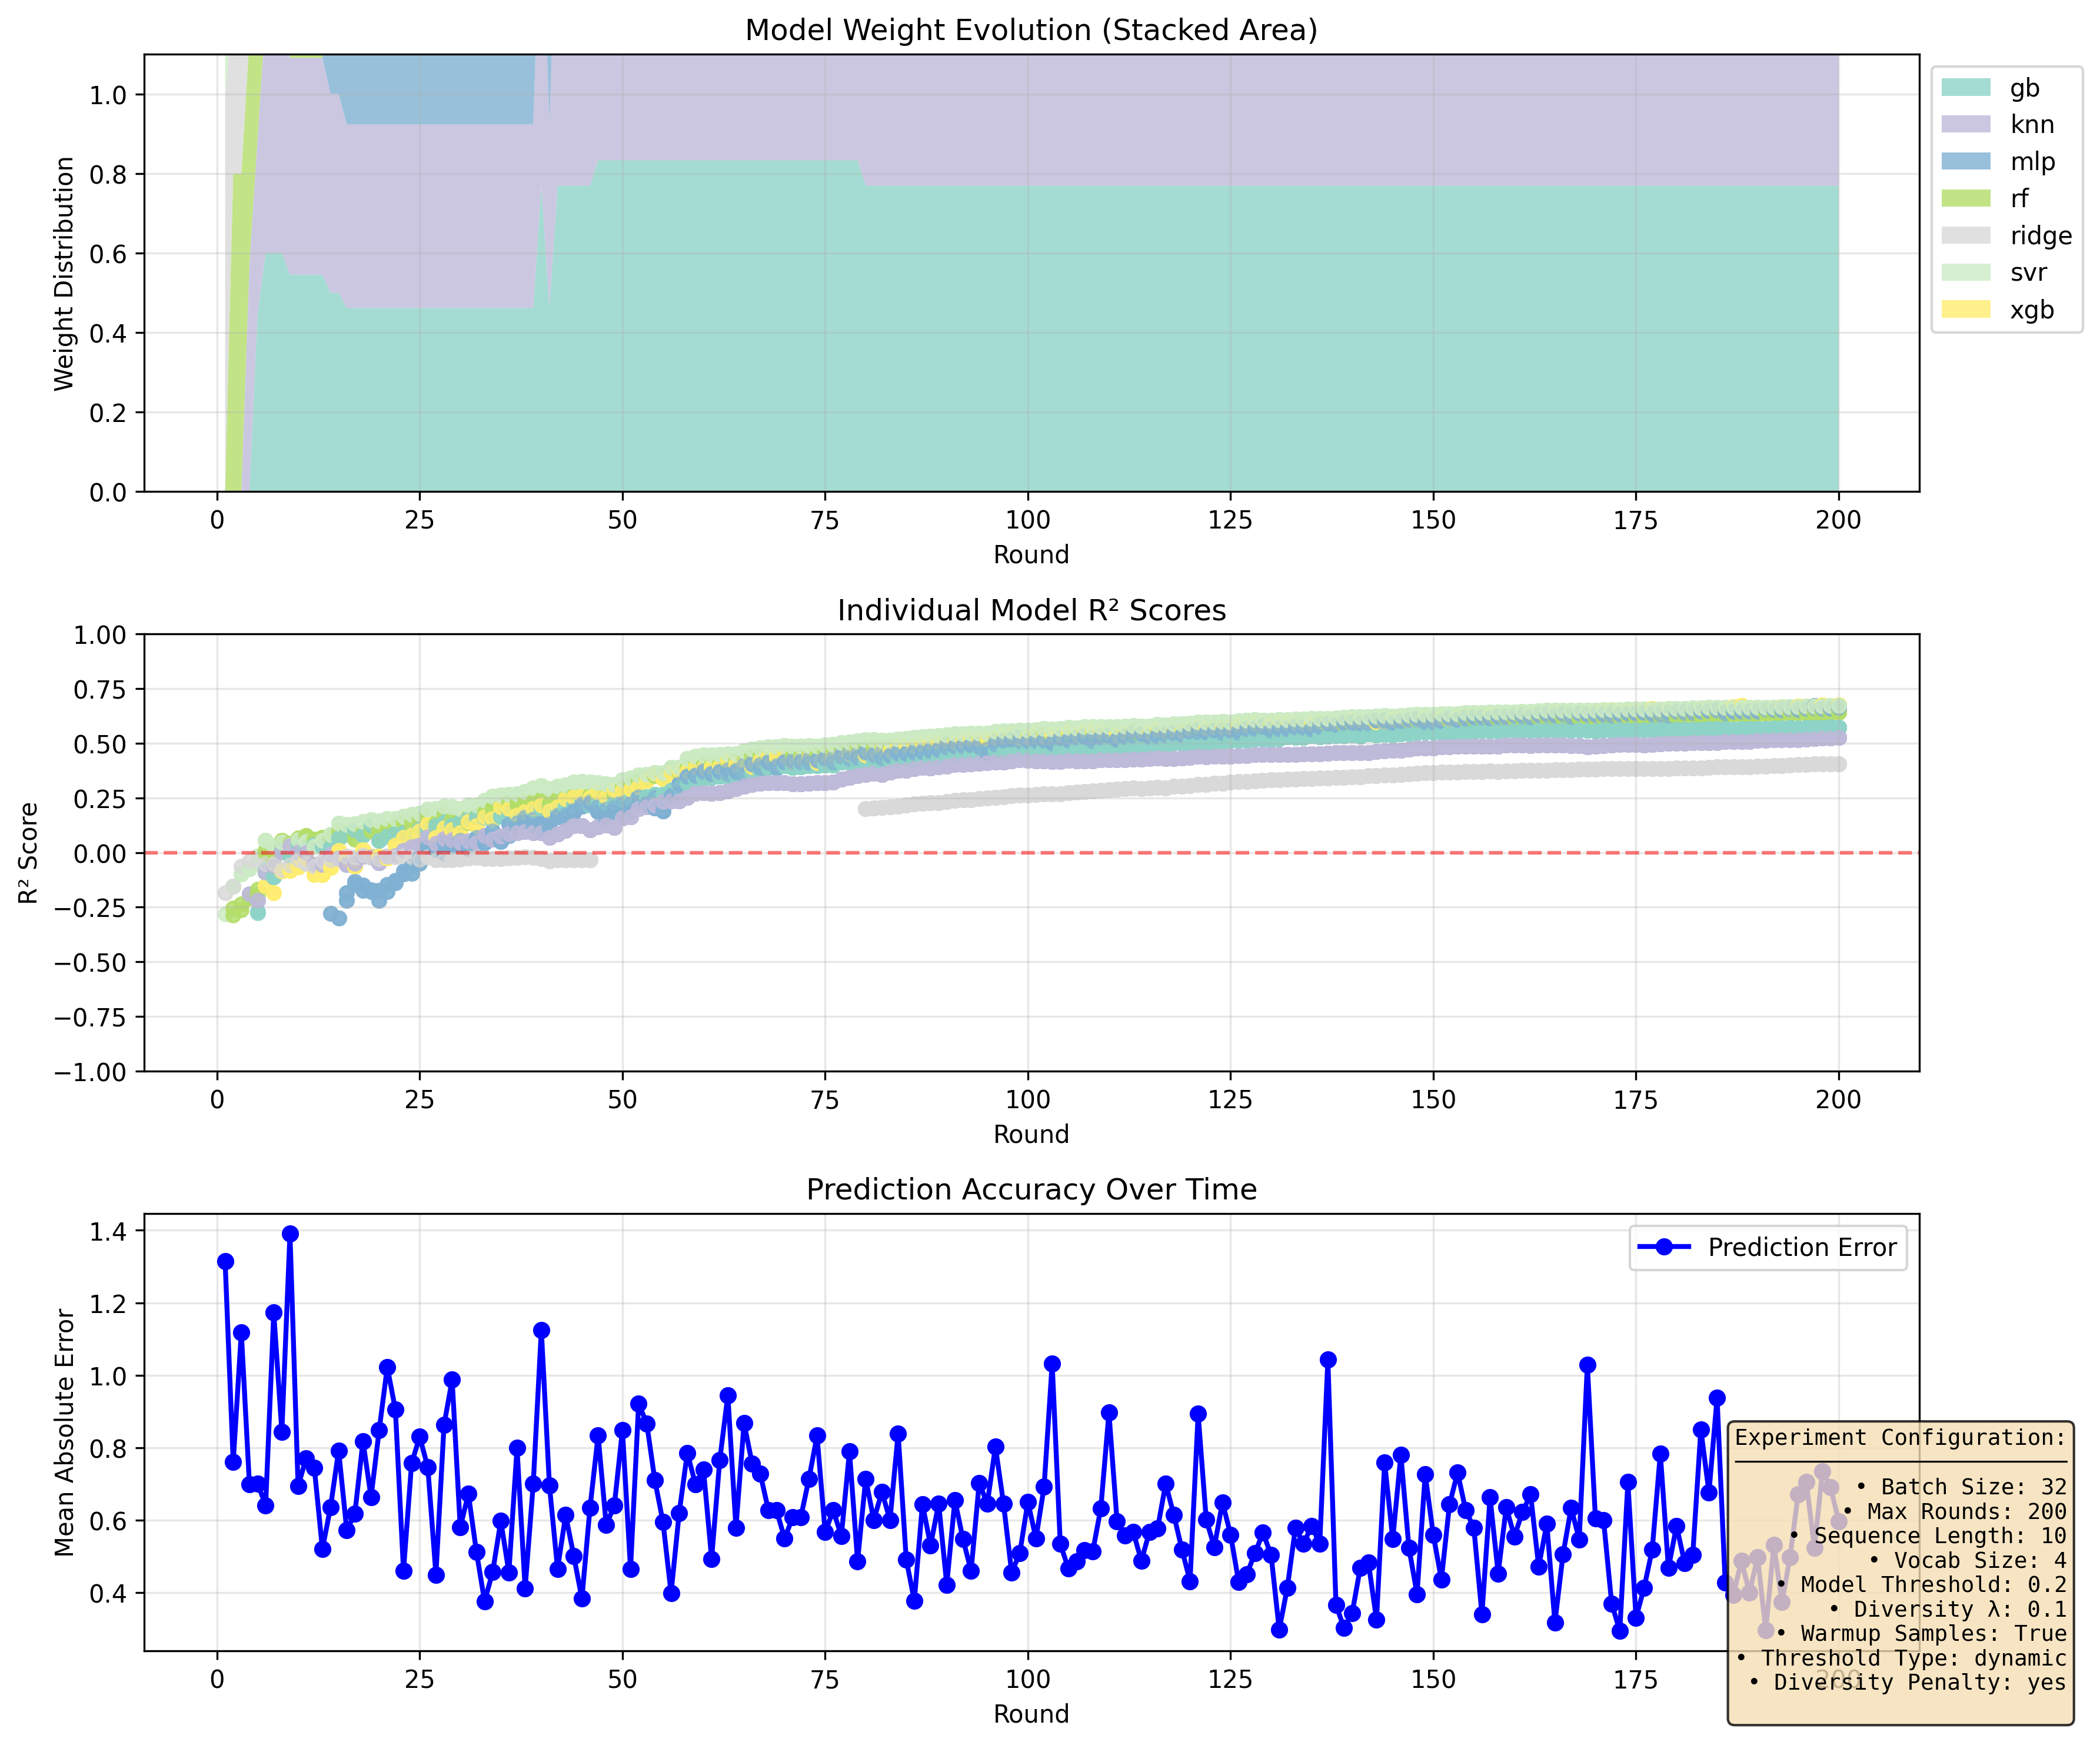
\includegraphics[width=\linewidth]{images/model_evolution_r200_b32_l10_average.png}
        \caption{Average Ensemble}
        \label{fig:average_model}
    \end{subfigure}
    
    \vspace{1em} % optional vertical space

    \begin{subfigure}[b]{0.8\linewidth}
        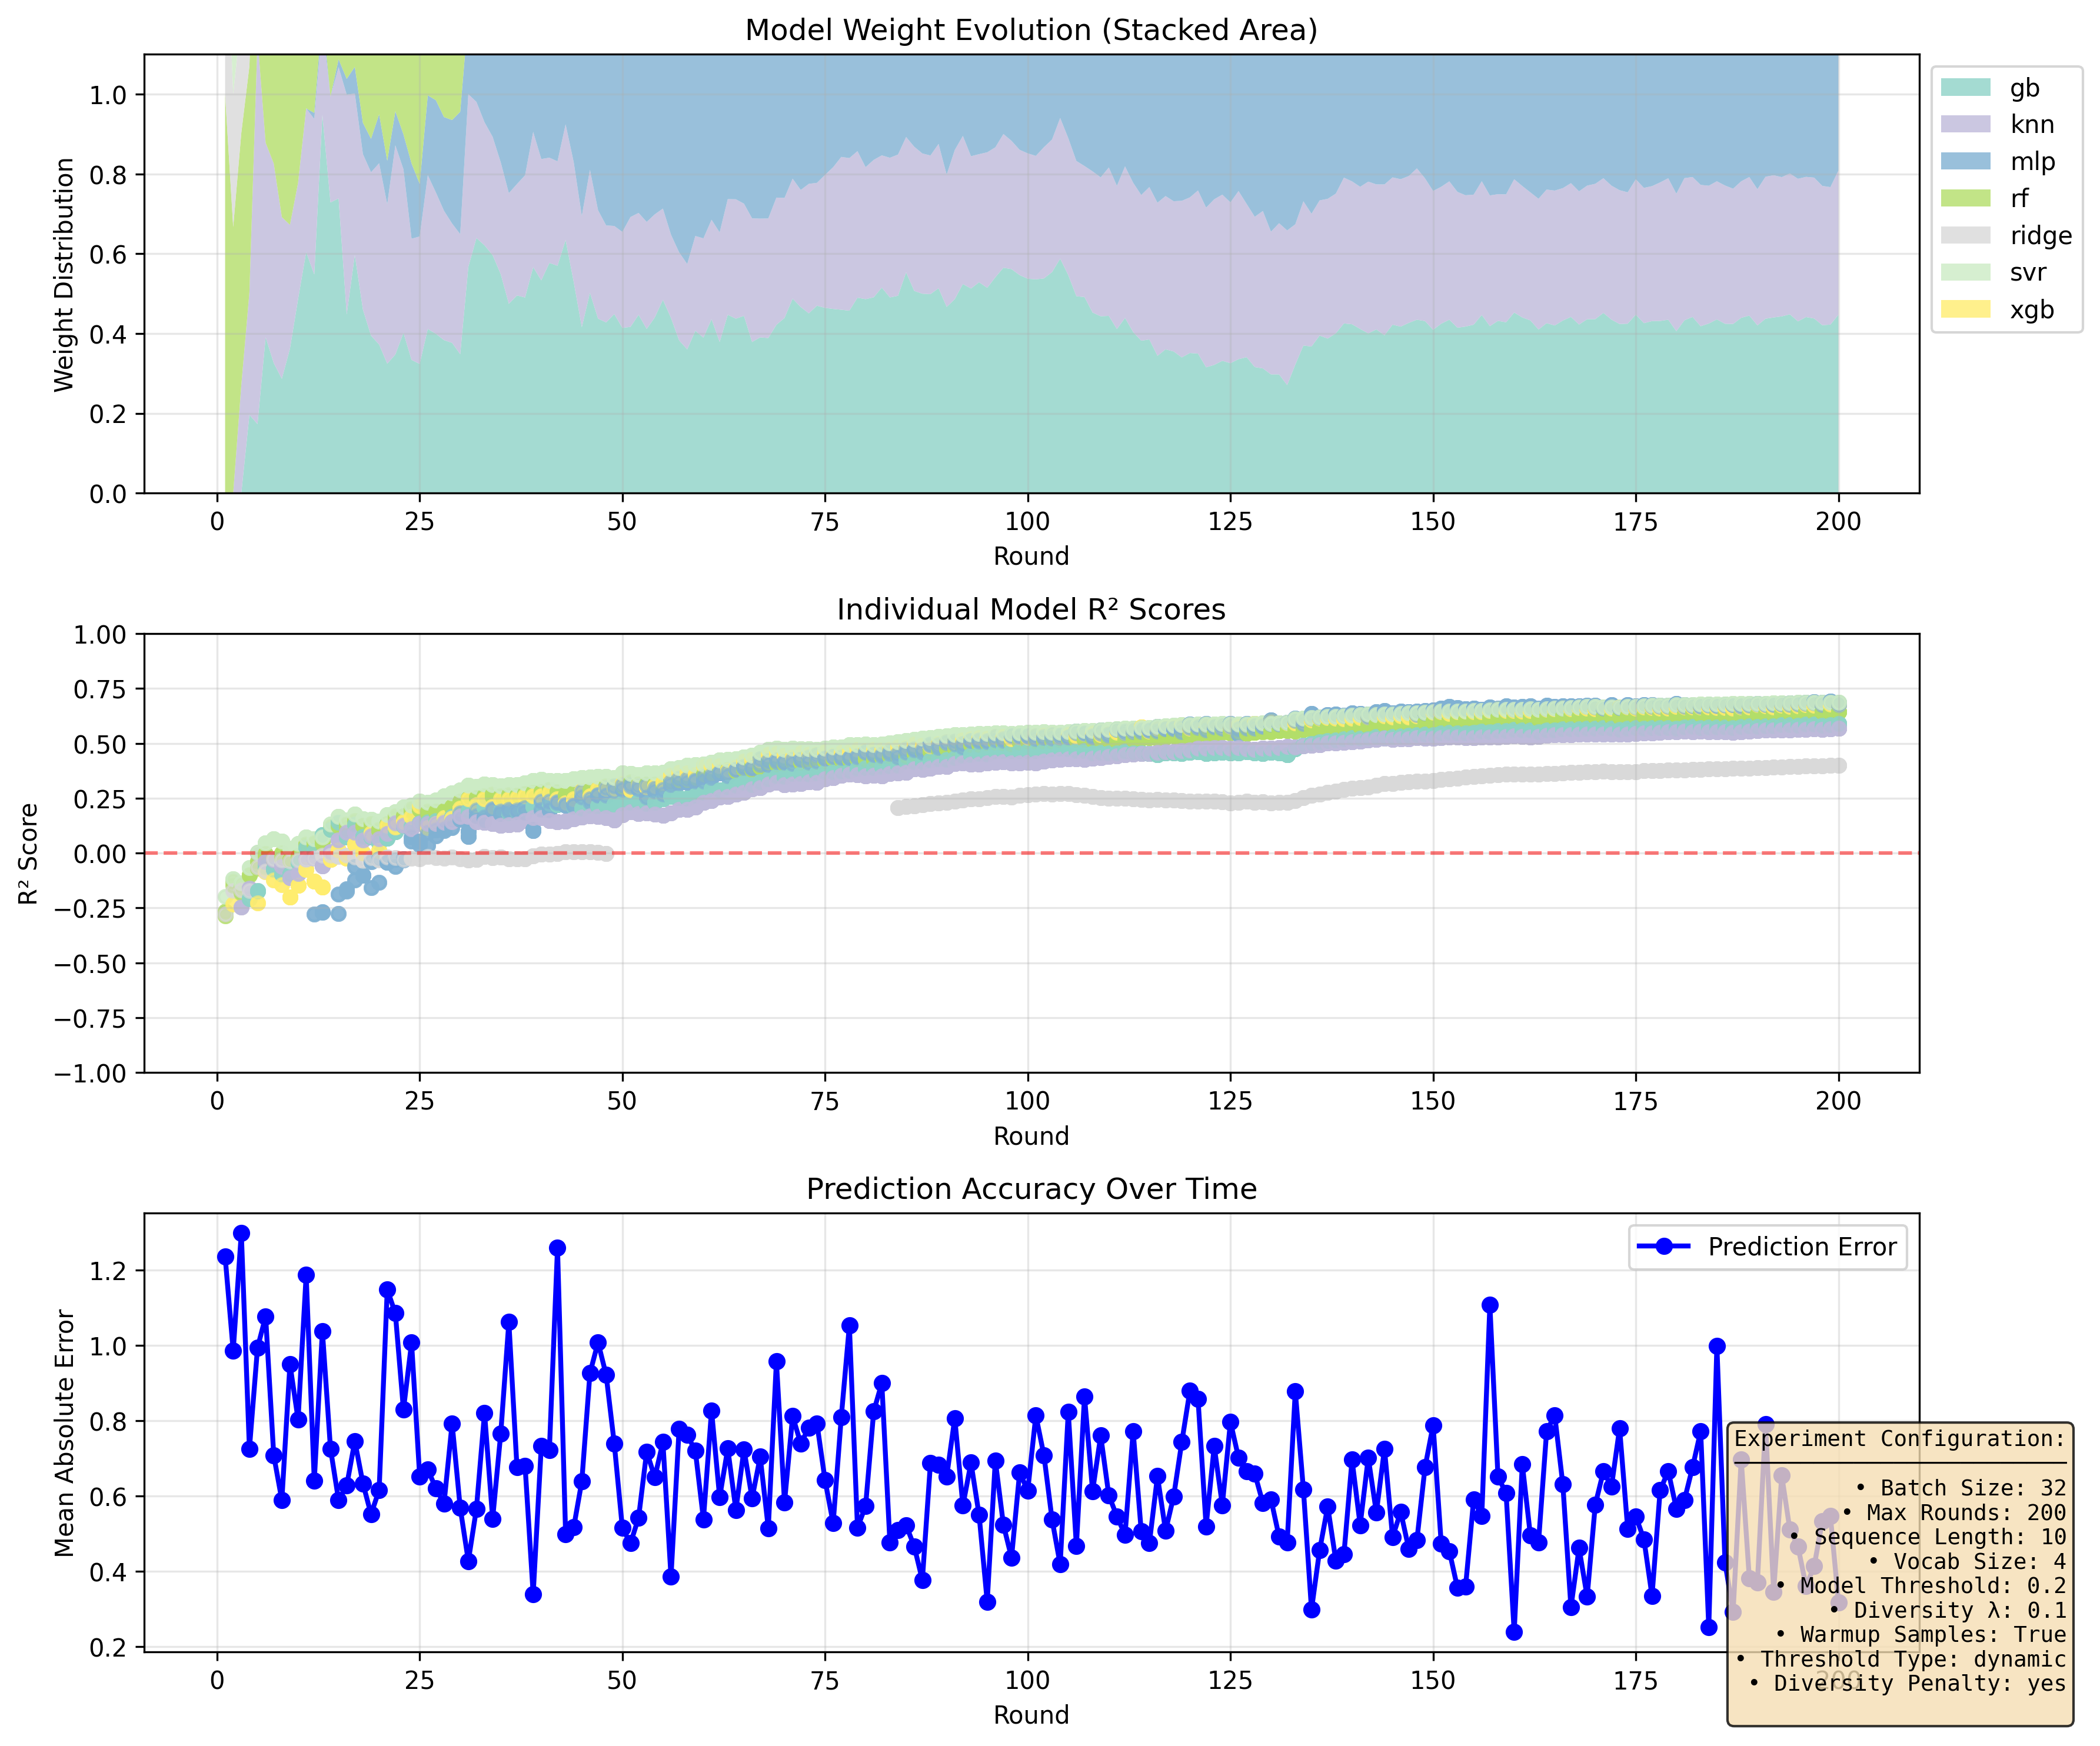
\includegraphics[width=\linewidth]{images/model_evolution_r200_b32_l10_weight.png}
        \caption{R2 Weighted Ensemble}
        \label{fig:weight_model}
    \end{subfigure}
    
    \vspace{1em}

    \begin{subfigure}[b]{0.8\linewidth}
        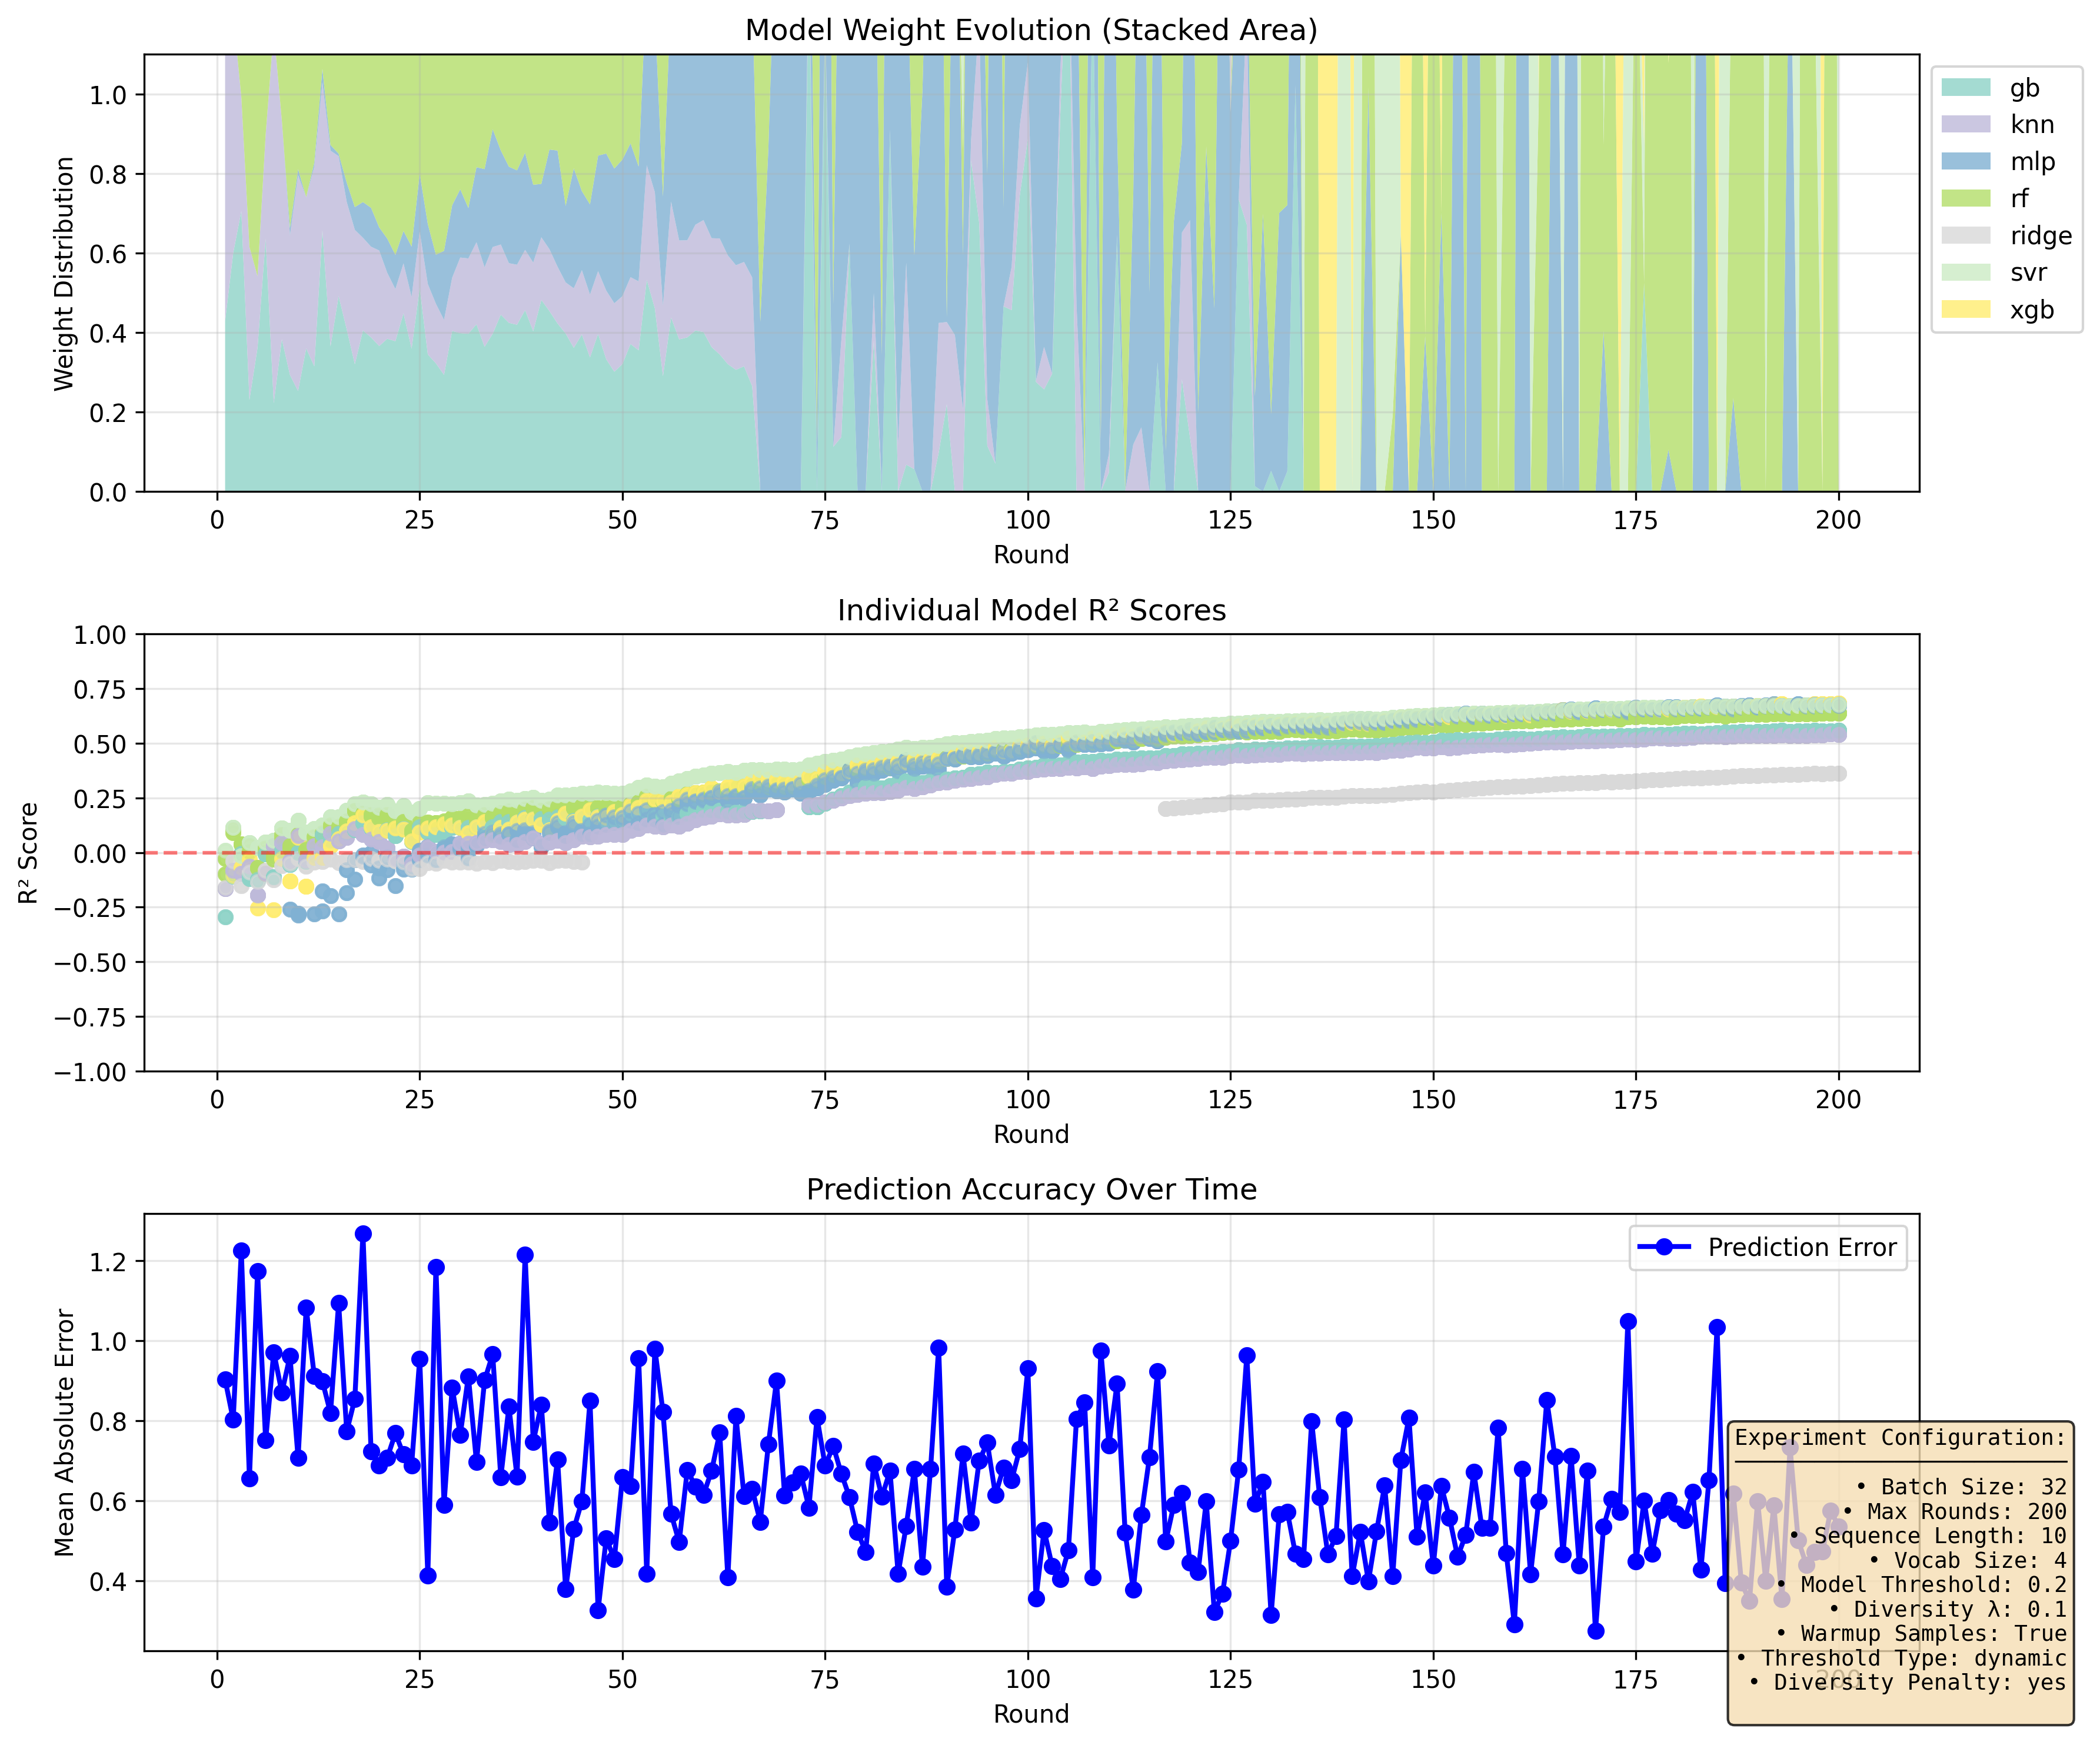
\includegraphics[width=\linewidth]{images/model_evolution_r200_b32_l10_dynamic.png}
        \caption{Dynamic Ensemble}
        \label{fig:dynamic_model}
    \end{subfigure}

    \caption{Model evaluation of three ensemble approaches.}
    \label{fig:model_evaluation_basic}
\end{figure}






\begin{comment}
\subsection{Base Comparison}
We compare the following approaches:
\begin{itemize}
    \item Standard with average ensemble
    \item R\textsuperscript{2}-based weighted ensemble
    \item Dynamic optimal ensemble
    \item Pure PPO
\end{itemize}







Metrics to track:
\begin{itemize}
    \item Final best reward achieved
    \item Convergence speed (rounds to reach 90\% of best)
    \item Reward Variance
\end{itemize}
\end{comment}

\subsection{Ablation Study}
We test the importance of each component by removing them individually.  
Configurations:
\begin{itemize}
    \item no\_warmup
    \item no\_diversity\_penalty
    \item fixed\_threshold
    \item uniform\_weights\_only
    \item no\_context\_encoding
\end{itemize}



\subsection{Model Contribution Analysis}
We analyze the contribution of each model over time.  
For each round, we log:
\begin{itemize}
    \item Individual model R\textsuperscript{2} scores
    \item Assigned weights
    \item Prediction accuracy
\end{itemize}

Visualization: stacked area charts will show the weight distribution over time.






% Conclusion
\section{Conclusion}
Conclusion goes here.

\bibliographystyle{IEEEtran}
\bibliography{references} % You can create a references.bib file

\end{document}